\documentclass[onecolumn, draftclsnofoot, 10pt, compsoc]{IEEEtran}
\usepackage[margin=0.75in]{geometry}

\usepackage{cite}
\usepackage{graphicx}
\usepackage{setspace}
%\usepackage{tabularx}
%\usepackage{pgfgantt}
\usepackage{listings}

% 1. Fill in these details
\def \CapstoneTeamName{		Auction Hunter}
\def \CapstoneTeamNumber{		4}
\def \GroupMemberOne{			Alexander Hull}
\def \GroupMemberTwo{			Alexander Jacobson}
\def \GroupMemberThree{			Yufei Zeng}
\def \CapstoneProjectName{		Auction Hunter}
\def \CapstoneSponsorCompany{	}
\def \CapstoneSponsorPerson{		Ryan Kalb}

% 2. Uncomment the appropriate line below so that the document type works
\def \DocType{		%Problem Statement
				%Requirements Document
				%Technology Review
				Design Document
				%Progress Report
				}
			
\newcommand{\NameSigPair}[1]{\par
\makebox[2.75in][r]{#1} \hfil 	\makebox[3.25in]{\makebox[2.25in]{\hrulefill} \hfill		\makebox[.75in]{\hrulefill}}
\par\vspace{-12pt} \textit{\tiny\noindent
\makebox[2.75in]{} \hfil		\makebox[3.25in]{\makebox[2.25in][r]{Signature} \hfill	\makebox[.75in][r]{Date}}}}
% 3. If the document is not to be signed, uncomment the RENEWcommand below
%\renewcommand{\NameSigPair}[1]{#1}

%%%%%%%%%%%%%%%%%%%%%%%%%%%%%%%%%%%%%%%
\begin{document}
\begin{titlepage}
    \pagenumbering{gobble}
    \begin{singlespace}
    	
\includegraphics[height=4cm]{coe_v_spot1}
        \hfill 
        % 4. If you have a logo, use this includegraphics command to put it on the coversheet.
        %\includegraphics[height=4cm]{CompanyLogo}   
        \par\vspace{.2in}
        \centering
        \scshape{
            \huge CS Capstone \DocType \par
            {\large\today}\par
            \vspace{.5in}
            \textbf{\Huge\CapstoneProjectName}\par
            \vfill
            {\large Prepared for}\par
            \Huge \CapstoneSponsorCompany\par
            \vspace{5pt}
            {\Large\NameSigPair{\CapstoneSponsorPerson}\par}
            {\large Prepared by }\par
            Group\CapstoneTeamNumber\par
            % 5. comment out the line below this one if you do not wish to name your team
            \CapstoneTeamName\par 
            \vspace{5pt}
            {\Large
                \NameSigPair{\GroupMemberOne}\par
                \NameSigPair{\GroupMemberTwo}\par
                \NameSigPair{\GroupMemberThree}\par
            }
            \vspace{20pt}
        }
        \begin{abstract}
        % 6. Fill in your abstract    
        	This design document outlines the components of our Auction Hunter development project. The elements, relationships, and design concerns will be discussed for each. This will serve as a road map for the remainder of this project. 
        \end{abstract}     
    \end{singlespace}
\end{titlepage}

\newpage
\tableofcontents
\newpage

\section{Introduction}
\subsection{Purpose}
The purpose of this document is to outline the design choices for each component of our proposed product. 
\subsection{Scope}
Auction hunter will pull data from one or many salvaged car auctions, store and process the data, then intelligently display evaluations through a web interface. 
\subsection{Context}
Every month hundreds of crashed vehicles get put up for auction by insurance companies in the United States and abroad. Quantifying the potential value of a wrecked car is tedious; each must be manually evaluated. Auction Hunter will help users gather information about the value of salvage vehicles, and provide recommendations. Auction Hunter seeks to watch as many auctions as publicly available and create pricing trends across different types of crashes. By applying previously gathered data to new auctions, a prediction can be made on the expected return on investment of these wrecked cars. The program will iterate through auctions, gather data and images, then populate a UI with relevant information. This will allow the users of Auction Hunter to better understand the real value of a used car and even assist in buying one for a fair price.

\subsection{Definitions}
\begin{itemize}

\item Web Crawler - a program that systematically collects information off of the web. This can be used to compile information or data without requiring a human to manually navigate to each web page. 

\item Website UI - A privately or publicly hosted website which will use an internet browser to display information to a user. It serves as a way for humans to easily interpret information that is being collected and calculated upon in the back-end. 

\item Wrecked Car Auctions - Insurance companies will commonly create auctions to sell cars that have crashed or been badly damaged. The insurance company will pay out an insurance holder, or replace their car. Vehicles are commonly auctioned because insurance companies avoid repairing them due to high or variable repair costs. 

\item Highest Value Car - The cars being sold at auction have some intrinsic value. This could be the grand total of each individual part after labor has been accounted for. It could also be the total price of the car after necessary repairs have been performed. Since the cars are sold at auction, this price is more variable based on bidders' actions. An auction would be worth bidding on if the total value is greater than the current asking price. Since there are so many auctions, the best would be displayed first.

\end{itemize}

%Other technical definitions

\section{Stakeholders}
Our project stakeholders are Ryan Kalb, Oregon State University, our CS Capstone group 4. Ryan Kalb first proposed the product and basic design, so he is the primary project stakeholder. 

\section{Design Components}

\begin{figure}[ht]
\centering
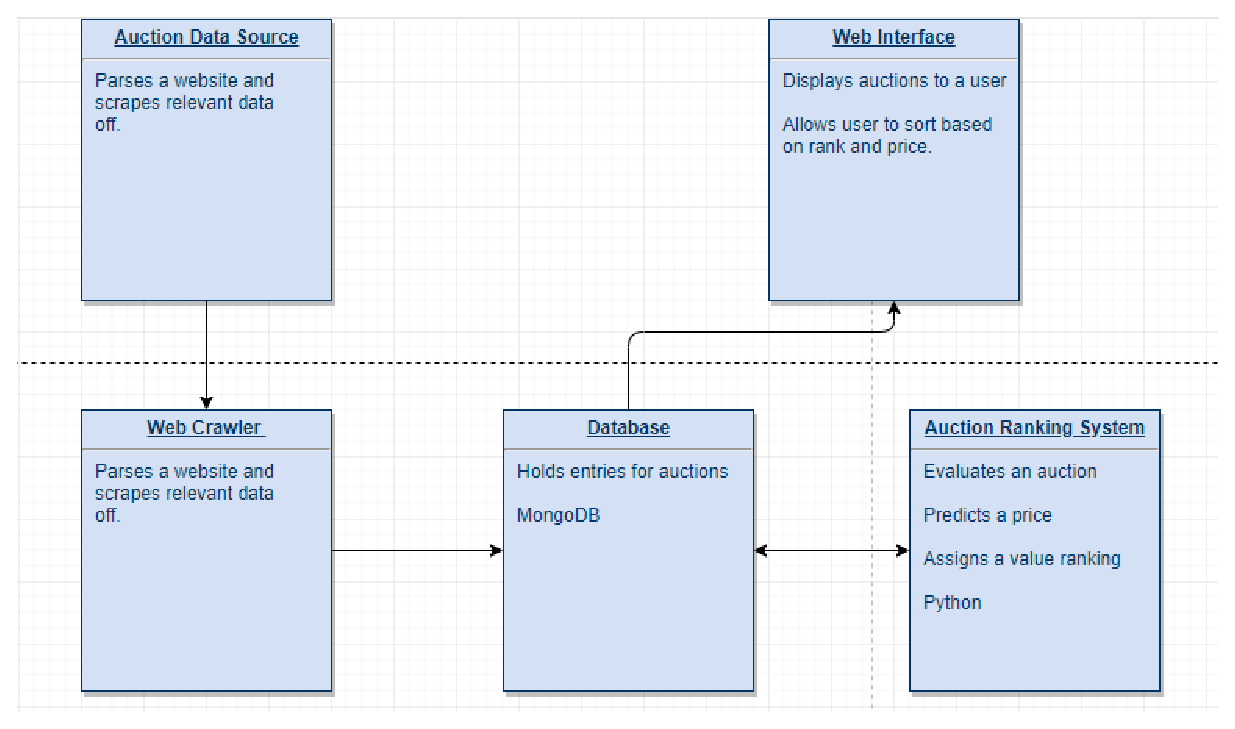
\includegraphics[scale=0.75]{flow_capture}
\caption{Flow Design}
\label{fig:flow}
\end{figure}


\subsection{Database Viewpoint}
\subsubsection{Design Description}
%Description of the design for a piece of the overall project
Our database will be implemented with the MongoDB database program.\cite{MongoDB} Each entry in the database will contain information on car from the auction website. Every relevant piece of information that is available on the website will be added to the database. Later, we can search though the database with a similar call: 
\begin{figure}[ht]
\centering
\begin{lstlisting}
db.collection.find( { price: { $gt: 10000 } } )
\end{lstlisting}
\caption{MongoDB 'find' example}
\end{figure}

This will return a structure with all the database entries with a price greater than \$10,000. 

\subsubsection{Design Elements}
%The elements that make up this viewpoint
There are two main elements to the Database design. The first is the database populator. The second is the database searcher. There is no need for the database to be updated after it has been populated, unless new entries are added for new auctions. However, our implementation could eventually extend to track auctions over time. In this case, we will add a list of variables such as price. This allows for static parameters to remain in the same database entry. For price, a list of price could be added which contains all updates to the price.


\subsubsection{Design Relationships}
The database populator will need to be closely coupled with the web crawler. The information scraped by the web crawler will need to be reconstructed into a document, then sent to the database with a MongoDB call.

\begin{figure}[ht]
\begin{lstlisting}
db.inventory.insertOne(
   { item: "Tesla Model S", price: 12500, tags: ["bumper damage"] }
)
\end{lstlisting}
\caption{MongoDB 'insert' example}
\end{figure}

The database searcher will need to be coupled with the auction ranking system as well as the web interface. Once all the information has been scraped off the auction websites, the local MongoDB database is the only thing the auction ranking system will need to have access to. The website will also access the database information, but might also link directly to the original website or images. 
%How the design interacts with other parts of the project


\subsubsection{Design Rationale}
%Explanation for the design that we are choosing, and the tools we are using
Modularity will make this project much easier to implement. By separating the populator and the searcher, we are able to split up the project into logical pieces. Since the web crawler only has access to the populator, and the auction ranking system only has access to the searcher, we enforce a strict process flow. 

\subsubsection{Design Concerns}
One concern is how we will implement a database that tracks the lifecycle of an auction. As stated earlier, there could be a list structure for dynamic parameters such as price to track over time. However, this would also require that the web crawler continually scrapes the website every time interval. This poses another issue where changes on the website could happen within minutes, especially when an auction is about to close. To continually check the website for updates, comparing the current parameters to the ones stored in the database, adds complexity to this problem. This issue might cause this implementation to exit the scope of this design. 
%Possible issues with design




\subsection{Website Viewpoint}
\subsubsection{Design Description}
%Description of the design for a piece of the overall project
The only and biggest portion of Auction Hunter that users will interact with is the website front end. Its job is to display the results of the web crawler and damage estimator. It also has to allow users to update and manage their preferences such as login information and auction notifications. The front end will actually be made up of two parts: client side and server side. Auction Hunter will use HTML/CSS and JavaScript to designed and build the client side code. The server side will be written in Python to receive the API calls from the client side. The client side code is what will make the site look nice, and be functional while the server side only has to respond to REST API calls and return the appropriate structured data to the client side for it to display to the user. When a user navigates to Auction Hunter in their web browser the client side code gets downloaded to their computer or mobile device and then is rendered in the browser. The client side code will then make requests to the server for different parts of data stored in the Auction Hunter database. The Python server side code receives those requests and the queries the database and returns the appropriate results. The server side code is in charge of making sure the client is authorized to see the data and is not attempting to do something malicious like delete data that doesn't belong to that specific user. 

\subsubsection{Design Elements}
%The elements that make up this viewpoint
There are several pieces to the front end: the client JavaScript, the client HTML/CSS styling, and the server side Python backend. The HTML/CSS styling is what will make the site look nice and be easy to use. While the JavaScript and Python will work together to make the site functional. 

\subsubsection{Design Relationships}
%How the design interacts with other parts of the project
The client side code will be served by a webserver hosted on the dedicated server Auction Hunter is using for hosting. The webserver will also act as a gateway to the Python server side code which will in turn make database queries to the mongoDB database also hosting on the dedicated server. 

\subsubsection{Design Rationale}
%Explanation for the design that we are choosing, and the tools we are using
The reason for splitting up the design and the functionality is so that the Auction Hunter team can work on those pieces independently. Once we get a basic working layout we can focus mostly on functionality. Once the core functionally is finished we can go back and update the styling to make it look nicer and be easier to use. JavaScript is required any time your doing something in a web browser as its the only scripting language that runs natively in all major browsers. Python is being used for the backend because the rest of Auction Hunter will be written in the same thing and the Auction Hunter team members are most familiar with it. 


\subsection{Web Crawler Viewpoint}
\subsubsection{Design Description}
%Description of the design for a piece of the overall project
For collecting car’s data, we need to find a method to collect the photo, bidding information, and winning bid amount of cars, and which are listed on eBay Motors, ADESA, Auction Auto Mall, Dashub, A better bid, Salvage bid, Smart Auction, OVE.com, Auto Trader, and Insurance Auctions USA Inc. Auction Hunter will allow users to integrate this information in one place. The potential solution is using website crawler technology to collect
the relative web images and data from the websites that were mentioned before. 
\subsubsection{Design Elements}
%The elements that make up this viewpoint
Web crawler is a kind of script which will follow a special set of rules to automatically gather information from a website. Web crawling is also called web scraping, or web spidering. It is used for web classification in World Wide internet. All kinds of search engines use web crawler to provide valuable searching results. In fact, web crawler collects some special HTML images or text contents or some hyperlinks from other website, and view them in an appropriate way. The scraping mainly includes two steps: The first one is that looking for and downloading web pages systematically. The second one is that extracting information from web pages we got in advance.
\subsubsection{Design Relationships}
%How the design interacts with other parts of the project
The data web crawler extracted will be reconstructed in some ways, and stored in database for future use.
\subsubsection{Design Rationale}
%Explanation for the design that we are choosing, and the tools we are using
Scrapy is a twisted-based Python frame work for web crawling .It can be used to parse or extract HTML,XML,JS and CSV style documents. The main function of it includes: Requests manager, Selectors and Pipelines. For pipelines, once we got the data from website, we are able to pass them through different pipelines. Such as storing the scraped data, cleaning the HTML data, and validating data. For selectors, it is Scrapy’s own mechanism, and it is used to extract data. Selector works by selecting the selected parts of HTML files which specified by the expressions of XPath and CSS.For requests manger, it is responsible for downloading pages, and it will work behind the event at the same time. That is the reason why Scrapy costs less time than other web crawler. Scrapy is compatibly with some complicated crawl scenes. For example, for Auction hunter, we need to crawl many pages from different website. Using Scrapy will be a good choice.





\subsection{Web Hosting Viewpoint}
\subsubsection{Design Description}
%Description of the design for a piece of the overall project
Auction Hunter is going to be hosted on a dedicated server located in one of the team member's houses. This server hosts several virtual machines (VM) one of which will be dedicated to hosting Auction Hunter. Auction Hunter will run on the latest Ubuntu LTS release for familiarity to all of the Auction Hunter team members. Inside that Ubuntu VM will be several Docker containers for the various parts of the website. Each part of Auction Hunter will be put into a Docker container and linked together using docker compose to form a complete working product.

\subsubsection{Design Elements}
%The elements that make up this viewpoint
The hosting consists of VMware's ESXi as the hypervisor running on the bare metal server with a Ubuntu LTS VM. In the VM Auction Hunter will use Docker to containerize each part of the system. There will be several containers including one for the front end, one for the backend, the web crawler, and the database. 

\subsubsection{Design Relationships}
%How the design interacts with other parts of the project
All code written for Auction Hunter will need a place to run. The dedicated hosting provided by one the team members will run every part of Auction Hunter, from the continuous integration system to the front end web server. All of these will live in Docker containers or as their own VM on the server. Each of the containers will be linked using Docker's networking features with the Nginx web server being the only end user facing portion. The web crawler will also access the internet to gather data but it won't be directly accessible by any of the users of Auction Hunter. 

\subsubsection{Design Rationale}
%Explanation for the design that we are choosing, and the tools we are using
The main reason for using dedicated hosting is it gives the Auction Hunter team the most control over how the different portions of the project interact. It also is the only completely free option, as the server is already online and in use. 


\subsection{Auction Ranking System Viewpoint}
\subsubsection{Design Description}
The auction ranking system is what will provide a best prediction for value, and which auction a user should focus on. Without this component, this project is simply a compilation and reorganization of auctions. The primary purpose is to generate a more realistic price prediction than the one listed on the website. The difference between the prediction and the listed price can allow a user to pick the highest value auctions. Additionally, some factors may matter more for a certain user, so tuning the value prediction based off those factors will provide a more realistic evaluation for that user.  
%Description of the design for a piece of the overall project

\subsubsection{Design Elements}
The Auction Ranking System will be implemented in python, and will require pulling data from our generated database. For each parameter stored in the database, a predicted value will be modified on the fly. For example, a single deployed airbag may subtract \$500 from the predicted price. The precise numbers will have to be tuned. A good starting point would be to attempt to predict a price as accurately as possible to the listed price based on all information from the website. Next, the tuning would be changed to favor certain parameters over others. The next element would be to send this information to the web view. This could be performed by adding a new entry to the database, or create a new database with relevant prediction information. An id would have to be created for both databases to be able to match entries between the two tables. 
%The elements that make up this viewpoint

\subsubsection{Design Relationships}
The auction ranking system will need interface primarily with the database created by the web crawler. This is where all the data comes from to feed into the algorithm. The second relationship is between the auction ranking system and the web interface. Tentatively, the auction ranking system will need to write to the database with its prediction values and rankings, to later be displayed by the website module. 
%How the design interacts with other parts of the project

\subsubsection{Design Rationale}
The auction ranking system will be written in Python because it interfaces the best with the other components. We use data to feed into the algorithm entirely from the database to make our implementation more modular and simplistic. Our stretch goal will be to track the entire life cycle of the auction, and compare our initial prediction to the final sale price. 
%Explanation for the design that we are choosing, and the tools we are using

\subsubsection{Testing}
To test our auction ranking system, we will perform value predictions on a set of auctions. Then, the predicted value can be compared to the asking price. The standard deviation can be found, which will give an indication of the accuracy. Predictions that are far from the asking price can be investigated further. If our auction ranking system is able to without flaw predict the same value as the asking price, there isn't much value to our product. Therefore, certain parameters can be weighted more heavily, and we can run the same value predictions over again and compare the old vs new predicted values. Some manual evaluation of the prediction will be necessary, which will help improve our algorithm. Our client Ryan Kalb should be capable of manually evaluating the price of an auction and then compare to our value.  

\subsubsection{Design Concerns}
A concern is how to send the result of the auction ranking system to the web interface. There are a number of ways to perform this, but they all break the clean modularity and sequence flow in place. 
%Possible issues with design




\subsection{Damage Estimation Viewpoint}
\subsubsection{Design Description}
%Description of the design for a piece of the overall project
As the bonus part of Auction Hunter, the purposes of developing damage estimation tool include that many consumers do not know the rough budget of repairing cost, and the cost of traditional manual screening method by machinist is too expensive and too ineffective. We hope to develop an EXUSCRC like accompanying tool on Auction Hunter to estimate the repair cost.   
\subsubsection{Design Relationships}
%How the design interacts with other parts of the project
The data damage estimation tool obtained will be reconstructed in some ways, and stored in database for future use.
\subsubsection{Design Rationale}
%Explanation for the design that we are choosing, and the tools we are using
On EXUSCRC site, user is asked to select the vehicle type by clicking a drop-down list first, because the vehicle type will determine paint cost, scratches repair cost, and dents repair cost. The second step is to select damage part by clicking areas on an image which shows damaged positions(front bumper, hood, right/left front bumper corner,  right/left fender, roof, trunk, rear bumper, right/left rear bumper corner, right/left rear corner bumper, right/left quarter panel, right/left front door, right/left rear door ,right/left front wheels, right/left rear wheels). Different damaged part of car will cause different cost. After selecting repair areas, the last step is that user is asked to answer if there are holes or dents existing on each damaged area, and their size. The above three steps can be done by anyone without car-repair knowledge in less than 2 minutes. After user finish the estimating, a repair estimate cost report will show immediately. In addition, the copy of image with damaged areas and cost report will be stored and attached to the corresponding car's data on Auction Hunter site as reference for other customers. Everyone is free to modify damaged areas and revise cost report for the specified car. It means everyone who visit our site is a potential contributor for damage estimation tool.     
\subsubsection{Design Concerns}
%Possible issues with design
The damage estimation tool did not count frame damage, however this kind of damage will significant increase repair cost. This tool only supports to estimate minor collision repair cost, and it cannot be used to estimate some invisible damage, like mechanical damage or salvage.



\subsection{Auction Data Source Viewpoint}
\subsubsection{Design Description}
The auction data source is where the auctions will be sourced from, and what the web crawler will be scraping data from. To create an effective tool, the maximum amount of information must be gathered from the website. Without sufficient information, we will have to rely more heavily on the users decision making. Considering this, IAAI.com \cite{IAAI} appears to be the best option 
%Description of the design for a piece of the overall project

\subsubsection{Design Relationships}
The choice of website will directly affect our implementation of the web crawler script. A stretch goal is to extend the functionality of the web crawler to other websites to be able to compile auction listings from multiple sources. 
%How the design interacts with other parts of the project

\subsubsection{Design Rationale}
IAAI has much more information than its counterparts, such as Copart \cite{copart}. There is information on where all damage takes place, as well as airbag status. It also has all data organized in plain text in one place, which will make web crawling much easier to implement. 
%Explanation for the design that we are choosing, and the tools we are using

\subsubsection{Design Concerns}
Using multiple data sources could pose a number of issues. One issue is since there is different information available from each website, it would be hard to make a 1:1 comparison between entries from two different sources. In addition, there are likely auctions that are posted on multiple websites. 
%Possible issues with design





\subsection{Collaboration Tools Viewpoint}
\subsubsection{Design Description}
%Description of the design for a piece of the overall project
The code repository can be seen like a file archive. The purpose of using code repository is to share code, and make a better software. A good code repository allows us easily version and share code with other developers,and a good collaboration software will raise our working efficiency.
\subsubsection{Design Elements}
%The elements that make up this viewpoint
We are going to use GitHub, Slack, and Discord to be our code repository and communication tool during this whole design cycle. 
\subsubsection{Design Rationale}
%Explanation for the design that we are choosing, and the tools we are using
The reason we are using GitHub to be our code repository is that When we are working on building Auction Hunter, we will produce many functions in progress. So we need to create a branch for the project, and any change we make won’t affect the master branch. We can feel free to commit changes on the branch.In addition, GitHub allows developer to track the changes done, we can easily find who made the change and when he made the change. And we are able to control the versions of project. If the newest version cannot be compiled, we can rollback to older version. Also, the function SCM of GitHub allows us to store the code in the same file without conflict.
The reason we are using Discord to be our communication tool is that it supports text chat, voice function, and file sharing at the same time. Slack is used to communicate and recieve announcement from our client.






\subsection{Continuous Integration System Viewpoint}
\subsubsection{Design Description}
%Description of the design for a piece of the overall project
The continuous integration system is a piece of software that allows for Auction Hunter to be tested and validated as it is being build. Every time code is pushed to the Git repository, in Auction Hunter's case, Jenkins will download it and run automated testing on it. Depending on the desire's of the developers it can also automatically deploy the code into the development or production environments. As team members start writing code, the Auction Hunter team will enforce a strict regiment of automatic tests. These tests will be created as features are added to the project to make sure any new additions don't break the whole system from functioning. Since there are many different parts of Auction Hunter each will have its own Jenkins project to contain the tests. Jenkins will be linked to our git repository so that all of the tests run whenever a developer creates a pull request. After a pull request is successful, Jenkins will then deploy the code to our development server to see the changes live. After manually testing the development version, developers can then create a pull request to the master branch which, after a successful pull request, will deploy the new changes to the production environment.

\subsubsection{Design Relationships}
%How the design interacts with other parts of the project
Deploying Jenkins onto the dedicated server is the main piece of the continuous integration system. It will need to be connected to the git repository where the Auction Hunter code is stored. It will also need to be able to talk to the Docker daemon that manages the Docker containers. In the git repository developers will need to create tests for Jenkins to run. Using Jenkin's built in Configurator, the Auction Hunter team will need to set up when and how the tests and developments are run.

\subsubsection{Design Rationale}
%Explanation for the design that we are choosing, and the tools we are using
Jenkins was chosen because continuous integration systems are very similar in their feature set and the team member of Auction Hunter are already familiar with this one. Setting up a continuous integration system is a complicated task and is different for every project, despite having some knowledge of how Jenkins work it will still be a learning process to get everything correct. Having some familiarity will save the team time at the beginning of the project so they can focus on coding and not messing around with tools. 


\newpage



\bibliographystyle{IEEEtran}
\bibliography{IEEEabrv,bib}


\end{document}
